%%%%%%%%%%%%%%%%%%%%%%%%%%%%%%
\section{本底检查}
选择好事例后,通过拟合$M_{\rm BC}$的分布可以提取信号个数。在这之前,先用单举的MC样本(Inclusive MC)来查看每一个单标记道的本底情况。
我们发现有一些衰变道遭受着来自具有相同末态的其他衰变道的污染,贡献为所谓的峰本底。
为了去掉这些本底,我们根据本底道的过程引进了一些本底道的特征变量,然后设置窗口从而将这些本底去掉。
具体的窗口要求列在表~\ref{tab:bkg}中。在单标记和双标记的时候都采用了这一去本底的窗口要求。
\begin{table}
  \begin{center}
  \footnotesize
   \caption{$\lambdacp$具有峰本底的衰变道和对应的本底过程及其去除方法。}
  \begin{tabular}{l|c|c}
      \hline \hline
       衰变道  & 本底过程& 去本底的方法 \\ \hline
       \multirow{2}{*}{$\modec$} & $\modebb$ & 要求$M(p\pim)$不在 $\Lambda$质量区间 $(1.11,1.12)\gevcc$内\\ \cline{2-3}
       & $\Sigma^+\pip\pim$ & 要求$M(p\pizero)$不在$\Sigmap$质量区间 $(1.17,1.2)\gevcc$内 \\ \hline
       $\moded$ & $\modedd$ & 要求$M(p\pim)$不在$\Lambda$质量区间 $(1.11,1.12)\gevcc$内 \\ \hline
       $\modedd$ & $\moded$ & 要求$M(\pip\pim)$不在$\Ks$质量区间$(0.48,0.52)\gevcc$内 \\ \hline
       $\modeccc$ & $\modea$ & 要求$M(\pizero\pizero)$不在$\Ks$质量区间$(0.48,0.52)\gevcc$内 \\ \hline
       \multirow{2}{*}{$\modeddd$} & $\modec$ &要求$M(\pip\pim)$不在$\Ks$质量区间$(0.48,0.52)\gevcc$内 \\ \cline{2-3}
       & $\modebb$ &  要求$M(p\pim)$不在 $\Lambda$质量区间$(1.11,1.12)\gevcc$内 \\ \cline{2-3}
    \hline\hline
   \end{tabular}
   \label{tab:bkg}
  \end{center}
  \end{table}
当采用了这一措施之后,我们可以看出已经没有了峰本底的影响。
图~\ref{fig:compare_dataMC}给出了Cocktail MC和数据的比较图,我们可以看到两者吻合的非常好。
此外,我们还定量地检查了cross feed过程影响。所谓的 cross feed 指的是这12个衰变道之间,其余11个衰变道对该信号道的污染情况。
我们定义两个变量:cross feed几率和cross feed数目比例,顾名思义,cross feed几率指的是11个本底衰变道被当作该信号道选进来的几率;
而cross feed数目指的是数据中11个本底衰变道被当作该信号道选进来的绝对的数目。
这两个量是严格相关的,cross feed数目取决于cross feed几率以及数据中该本底道的数目,我们按照我们测量的分支比以及cross feed几率来计算的cross feed数目,进一步的计算cross feed数目占该过程产额的比例。
这两个量都是有意义的,原则上cross feed数目比例是更有直接的参考意义的。
讲这些值和产额的统计误差比起来,我们可以看出峰本底已经被压低到了完全可以忽略的地步。

%%%%%%%%%%%%%%%%%%%%%%%%%%%%
\begin{figure*}[hp]
\centering
\subfigure[]
{
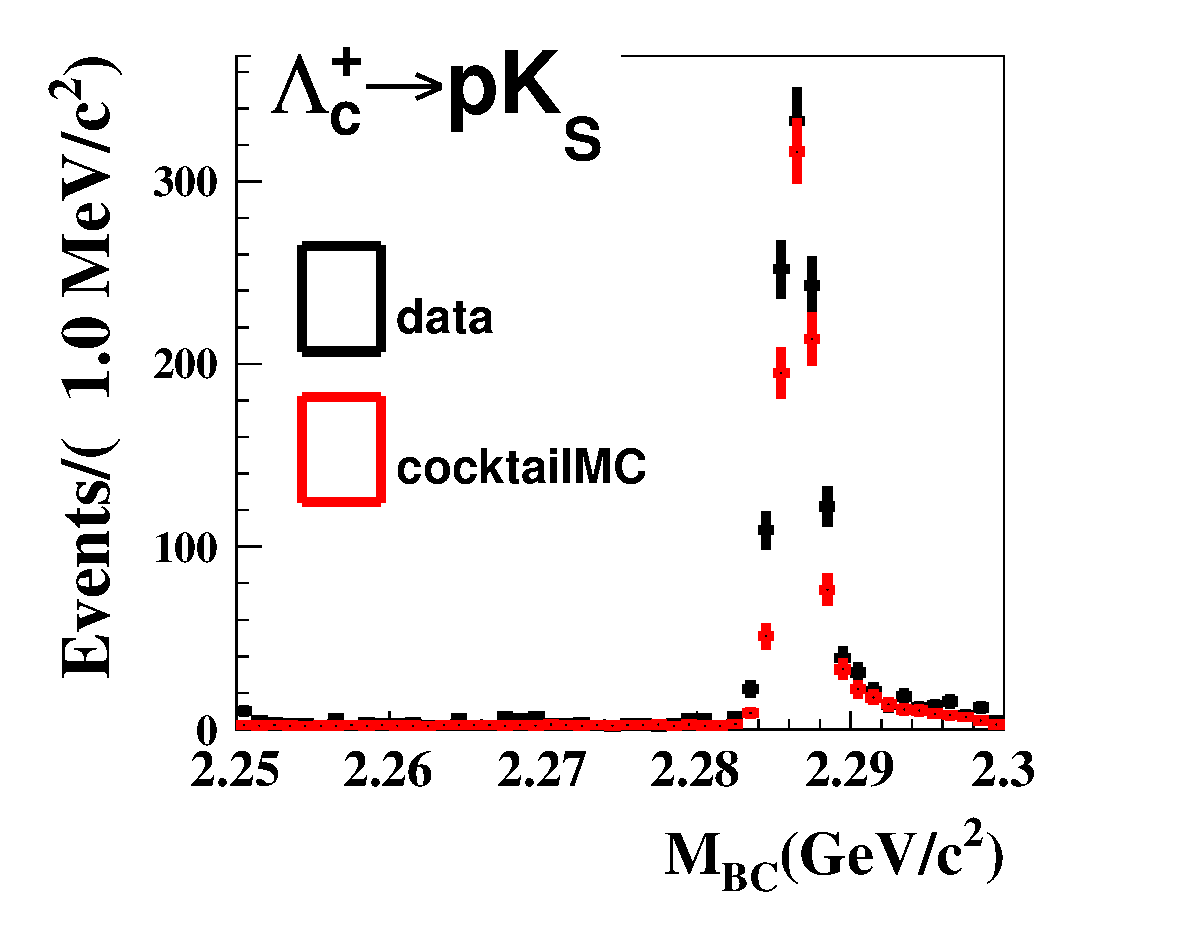
\includegraphics[width=0.3\textwidth]{chap2_compare_mode0}
}
\hspace{1pt}
\subfigure[]
{
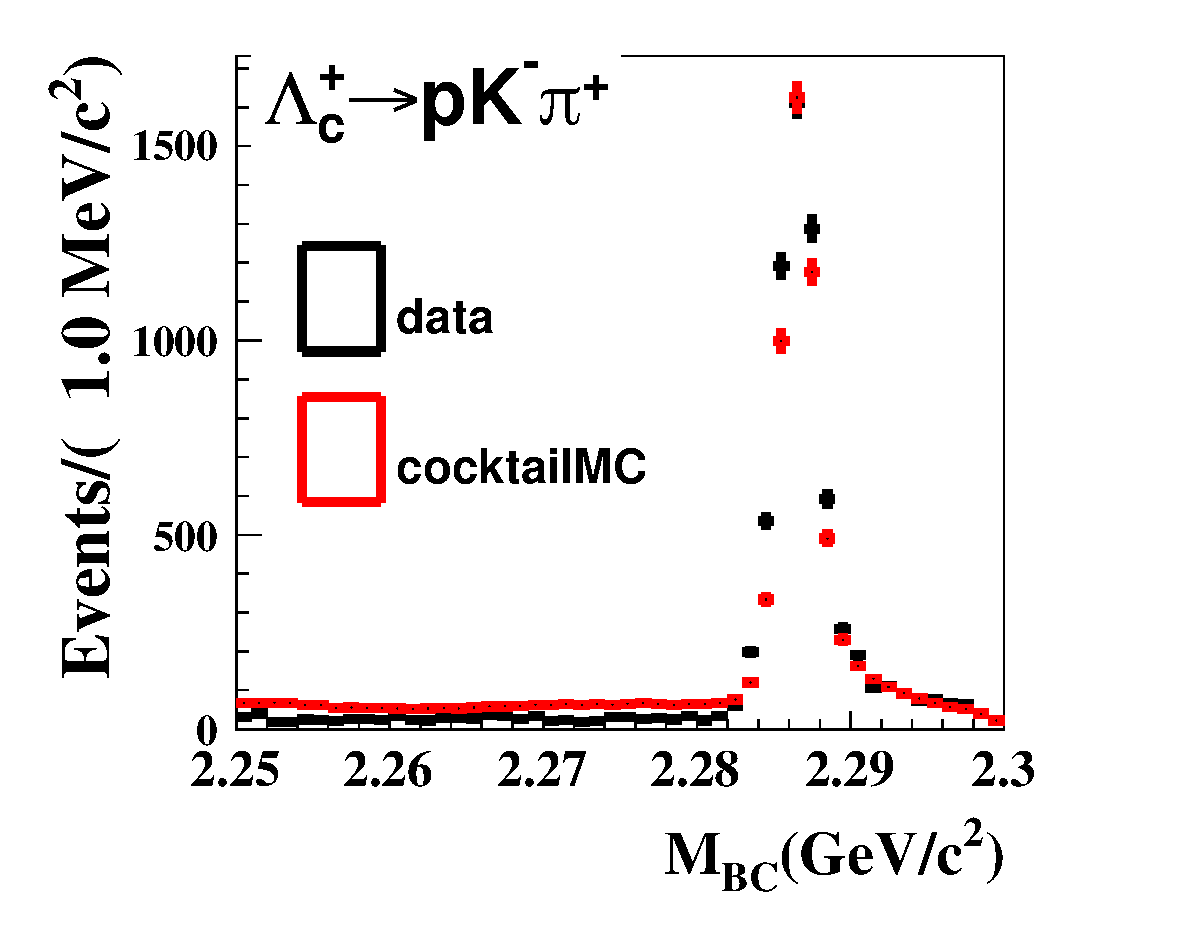
\includegraphics[width=0.3\textwidth]{chap2_compare_mode1}
}
\hspace{1pt}
\subfigure[]
{
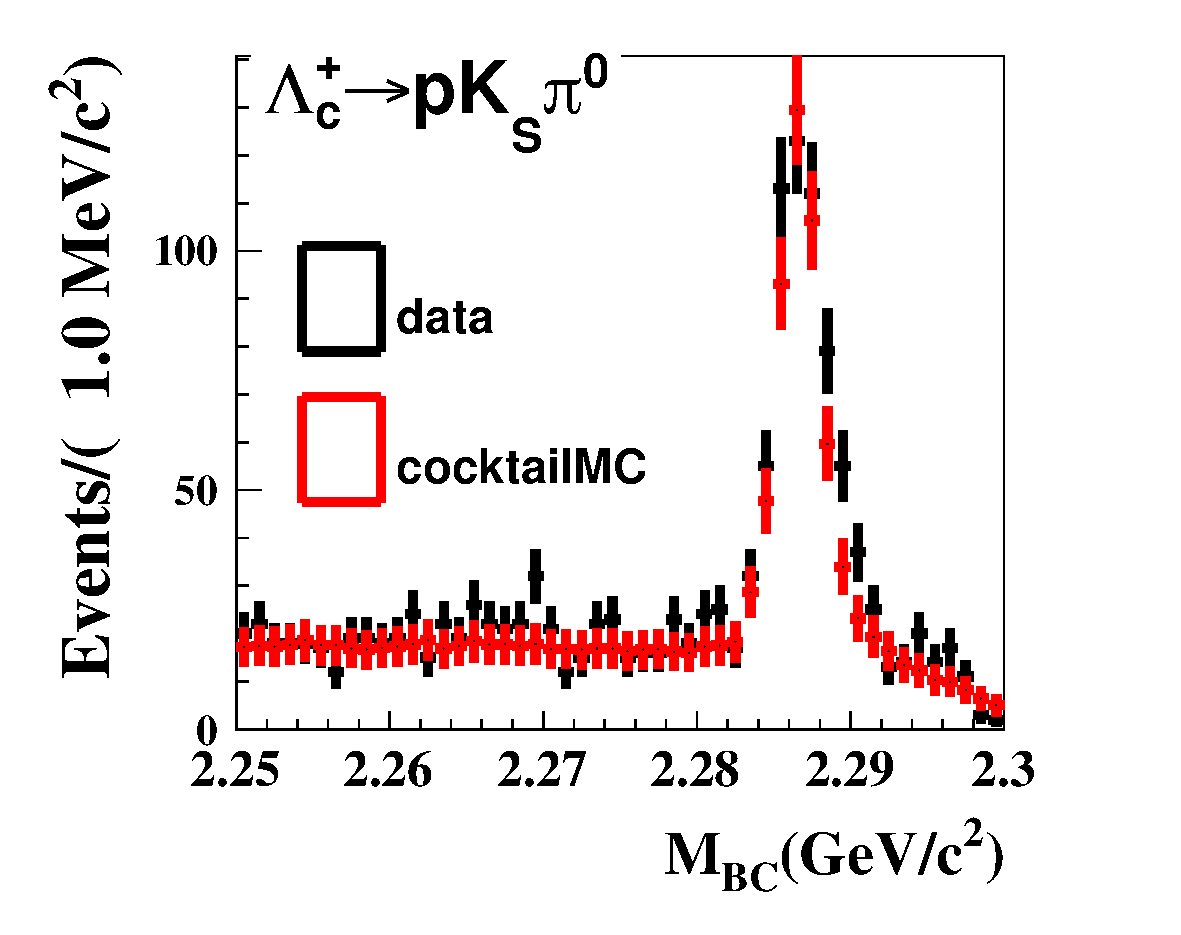
\includegraphics[width=0.3\textwidth]{chap2_compare_mode2}
}
\hspace{1pt}
\subfigure[]
{
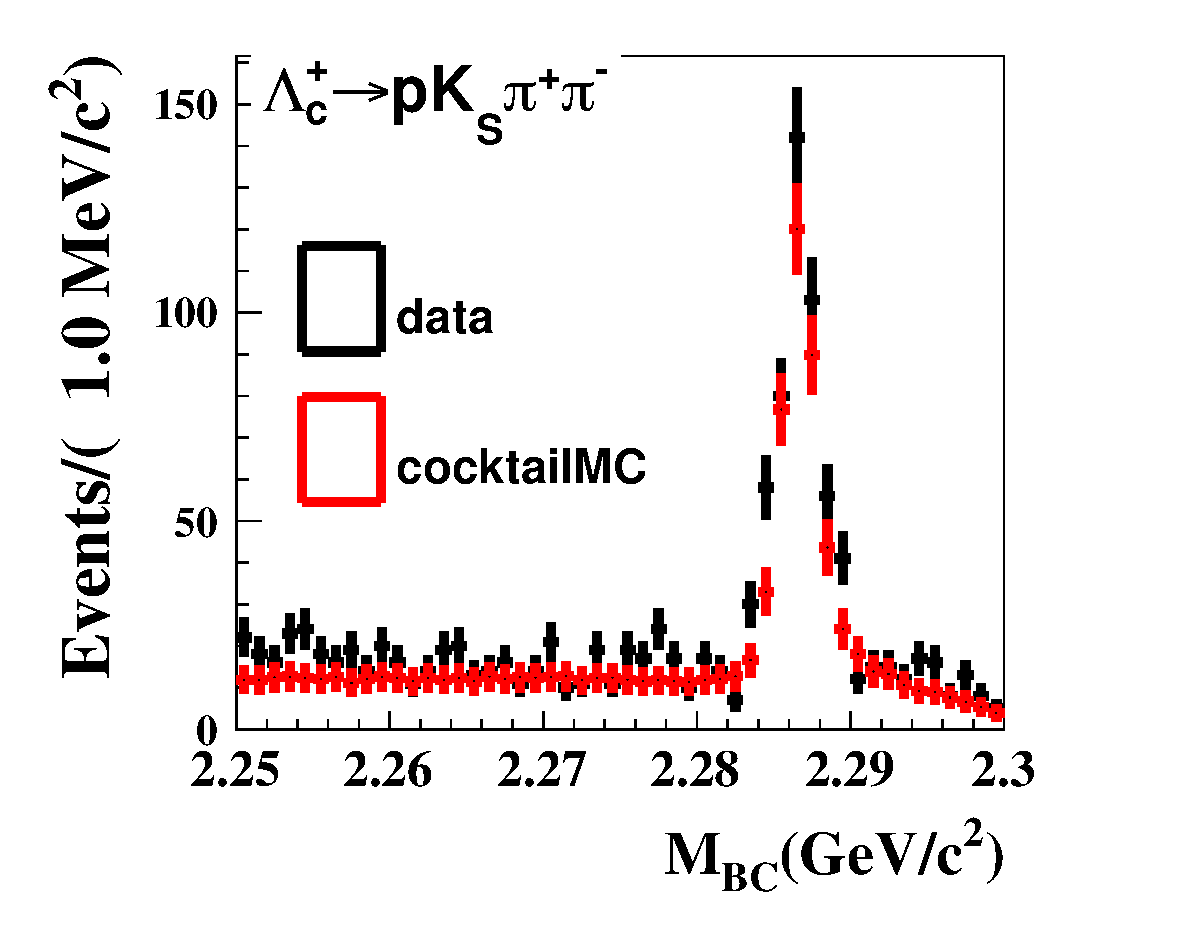
\includegraphics[width=0.3\textwidth]{chap2_compare_mode3}
}
\hspace{1pt}
\subfigure[]
{
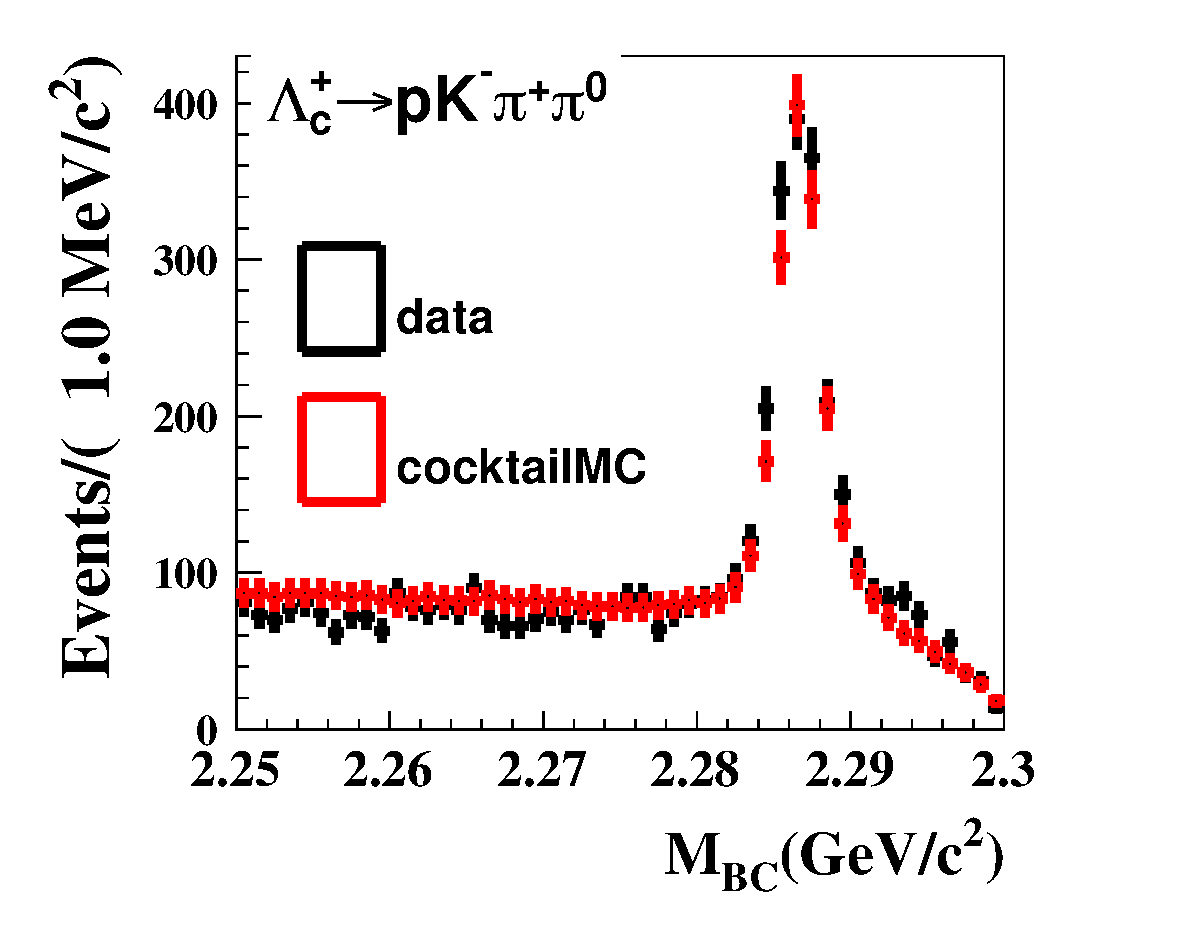
\includegraphics[width=0.3\textwidth]{chap2_compare_mode4}
}
\hspace{1pt}
\subfigure[]
{
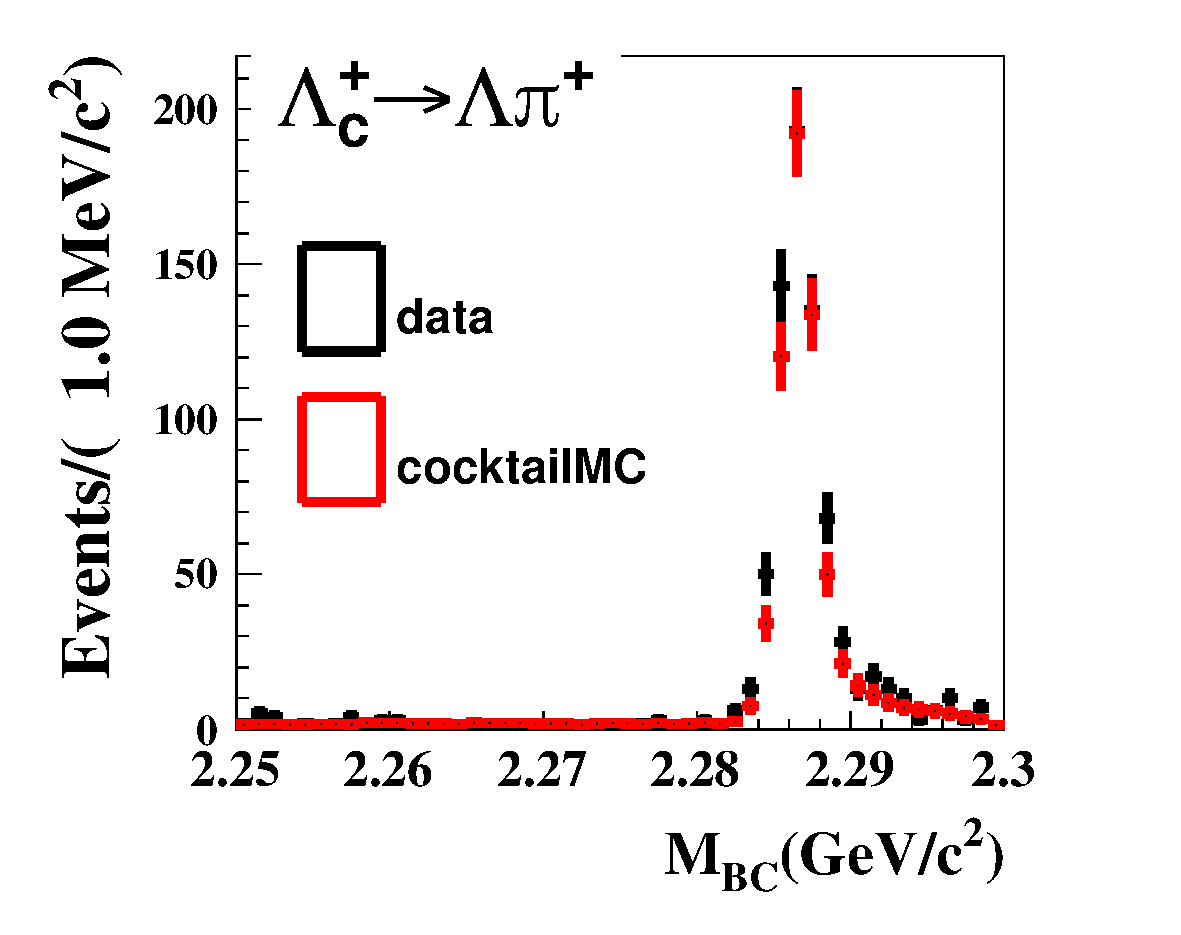
\includegraphics[width=0.3\textwidth]{chap2_compare_mode30}
}
\hspace{1pt}
\subfigure[]
{
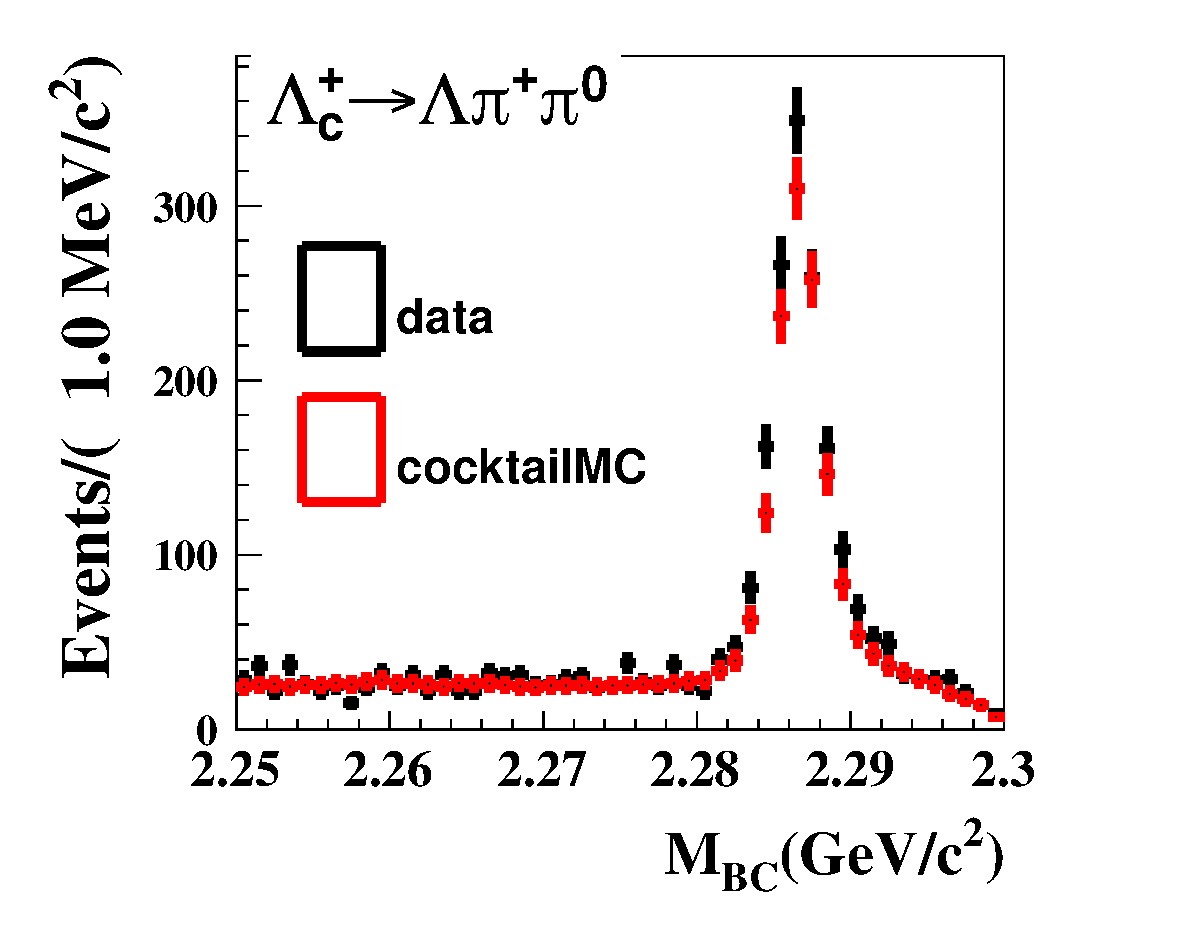
\includegraphics[width=0.3\textwidth]{chap2_compare_mode31}
}
\hspace{1pt}
\subfigure[]
{
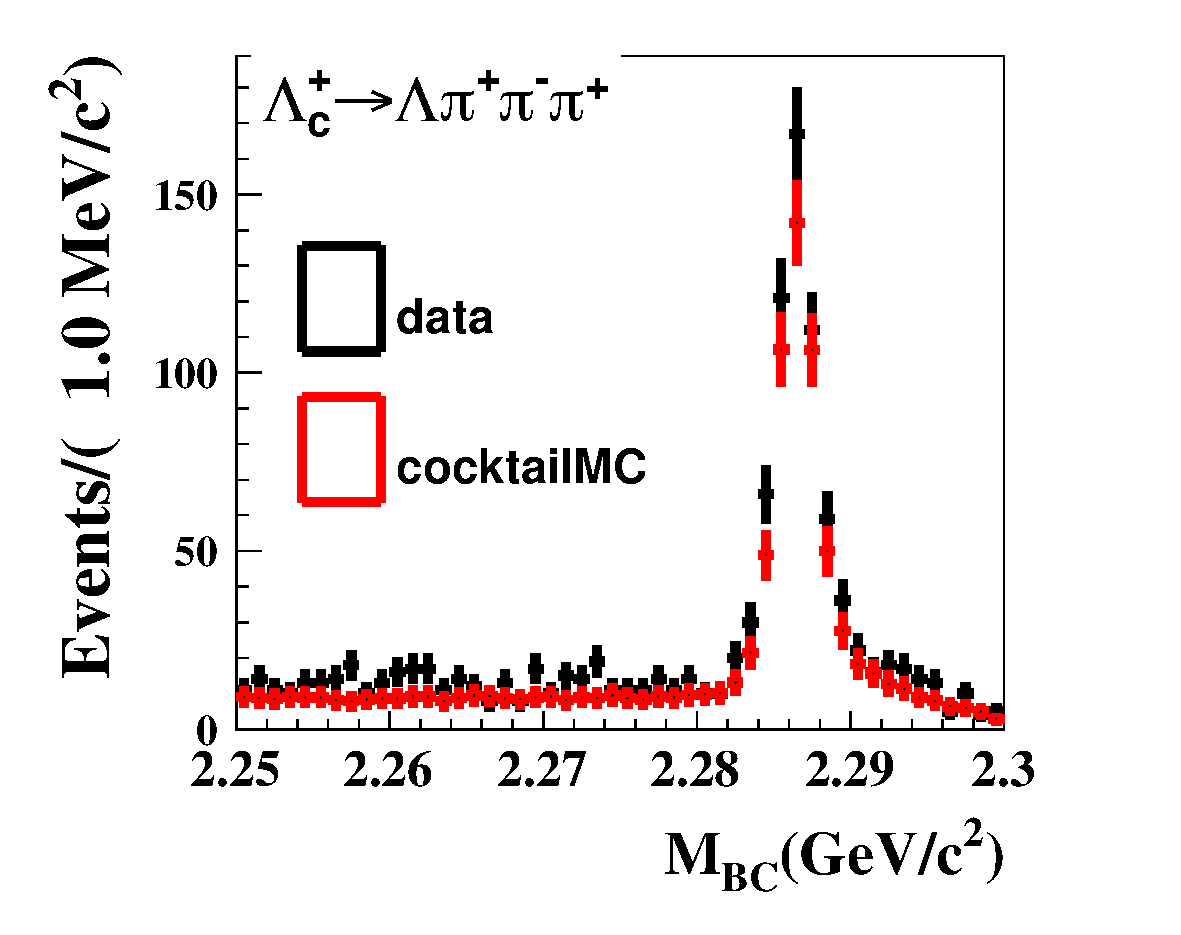
\includegraphics[width=0.3\textwidth]{chap2_compare_mode33}
}
\hspace{1pt}
\subfigure[]
{
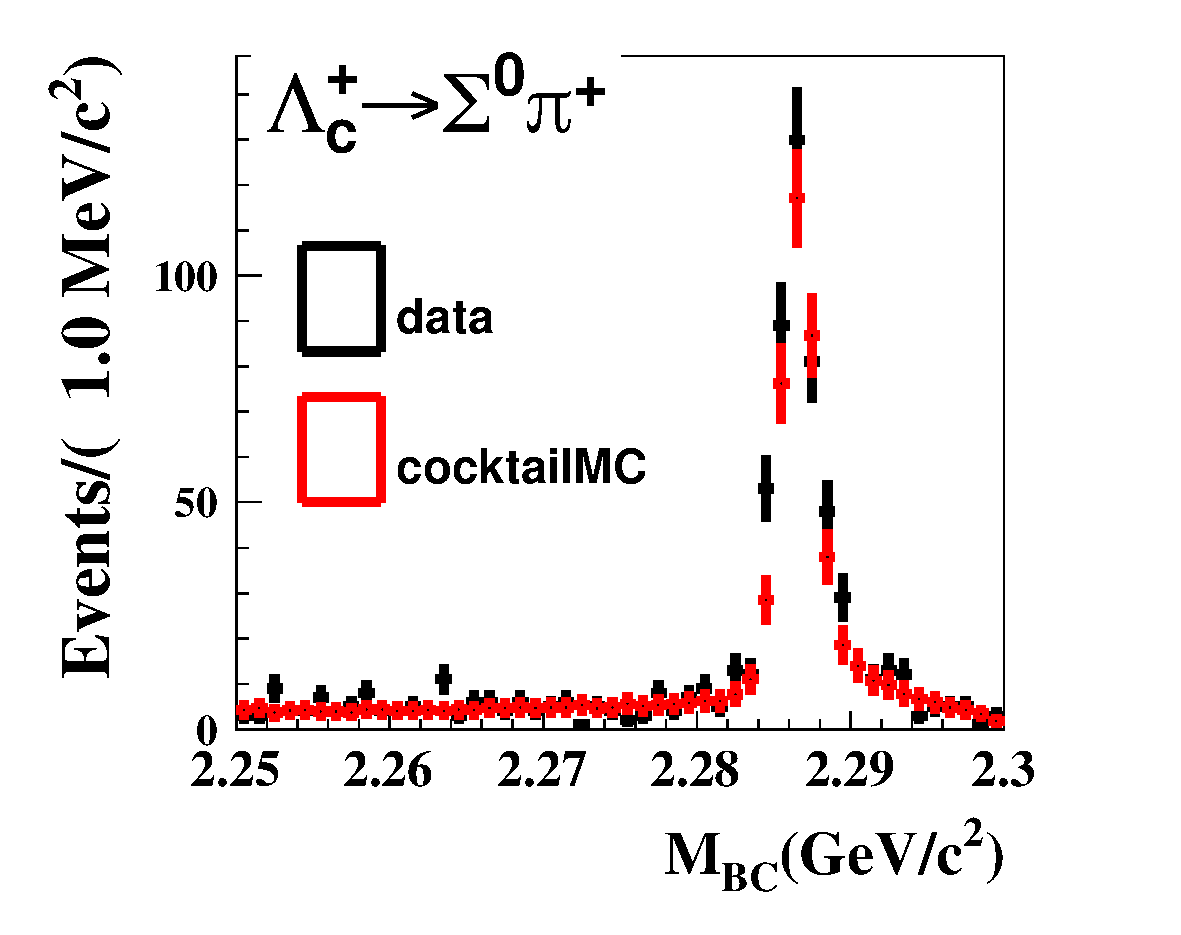
\includegraphics[width=0.3\textwidth]{chap2_compare_mode60}
}
\hspace{1pt}
\subfigure[]
{
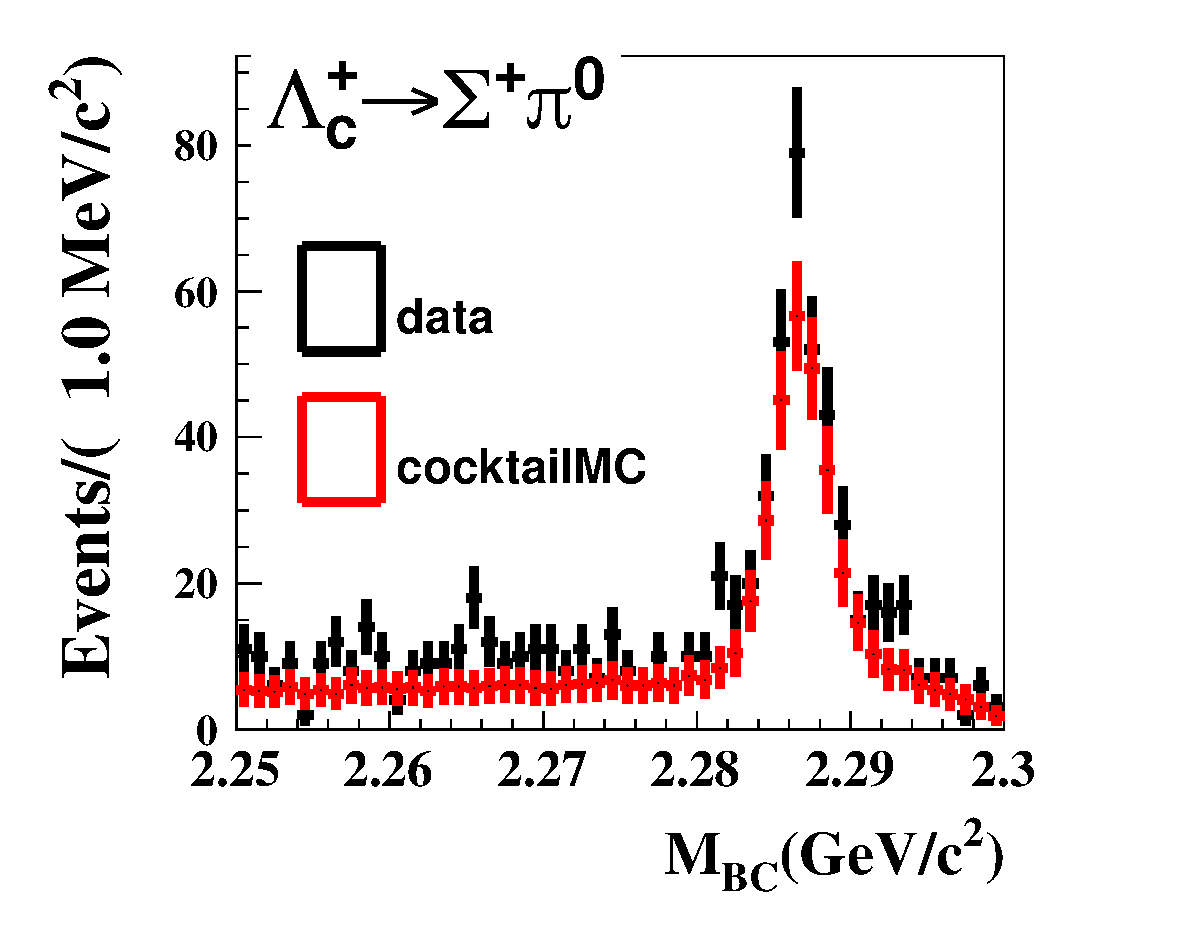
\includegraphics[width=0.3\textwidth]{chap2_compare_mode62}
}
\hspace{1pt}
\subfigure[]
{
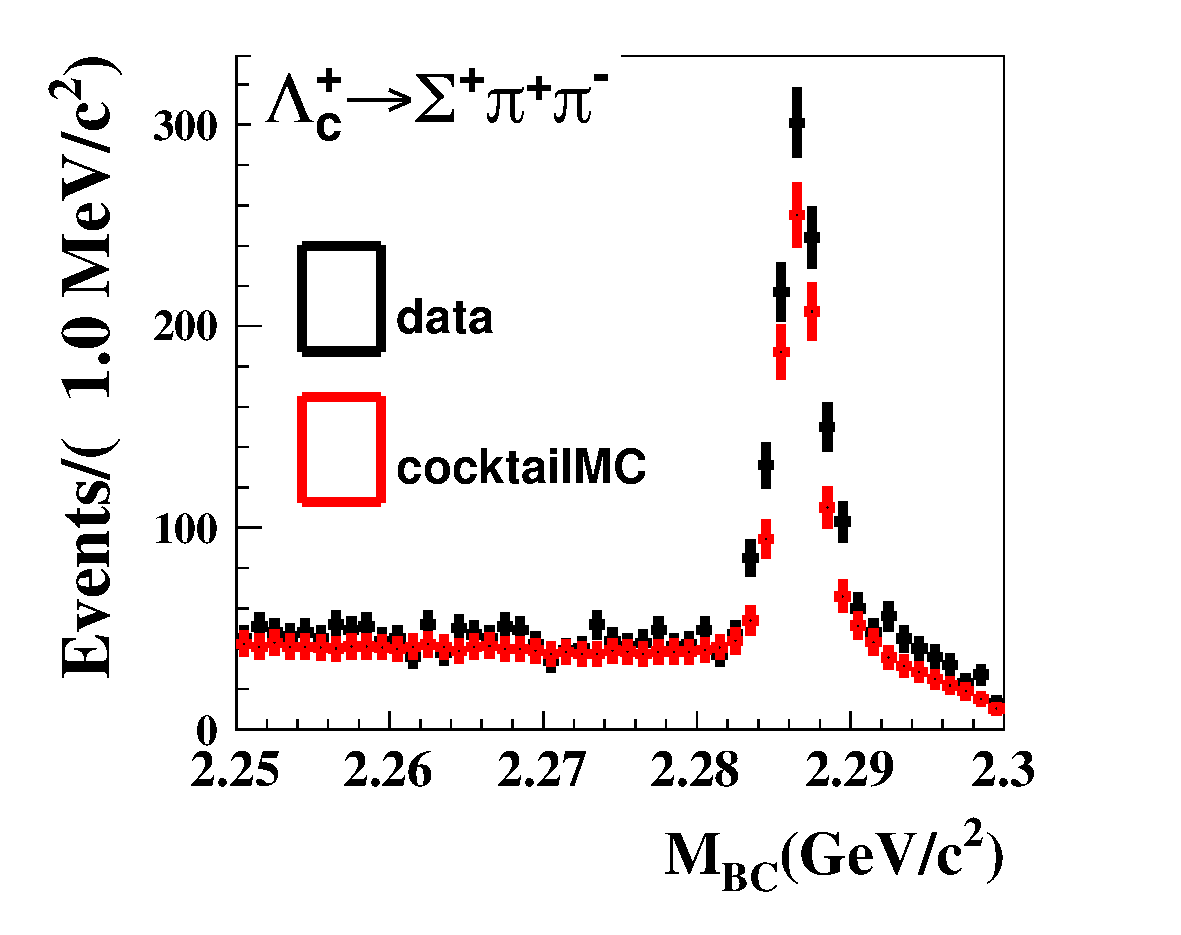
\includegraphics[width=0.3\textwidth]{chap2_compare_mode63}
}
\hspace{1pt}
\subfigure[]
{
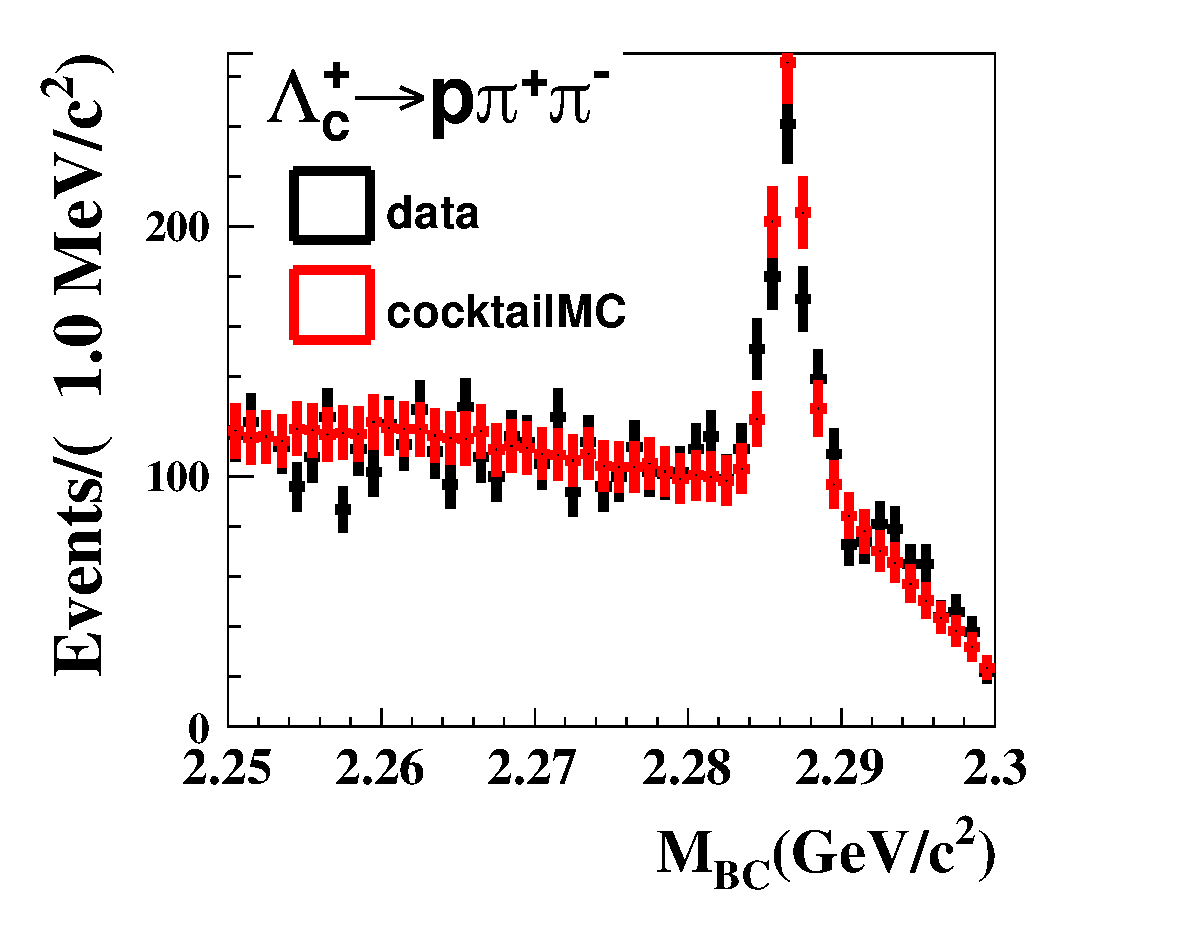
\includegraphics[width=0.3\textwidth]{chap2_compare_mode5}
}
\caption{Cocktail MC和数据的比较图。}
\label{fig:compare_dataMC}
\end{figure*}
